\chapter{Software Engineering}

\section{Introduction}

\subsection*{Software}
The Institute of Electrical and Electronic Engineers (IEEE) defines software as — \, a collection of computer programs, procedures, rules and associated documentation and data.

\vspace{1ex}
\begin{minipage}{0.6\textwidth}
   \subsection*{Software Product}
   Software, when made for a specific requirement is called software product. Software products may be —
   \begin{itemize}[parsep=1ex]
      \item \textbf{Generic:} developed to be sold to a range of different customers.
      \item \textbf{Customized (Bespoke)} developed for a single customer according to their specification.
   \end{itemize}
\end{minipage}\hfill
\begin{minipage}{0.38\textwidth}
   \centering
   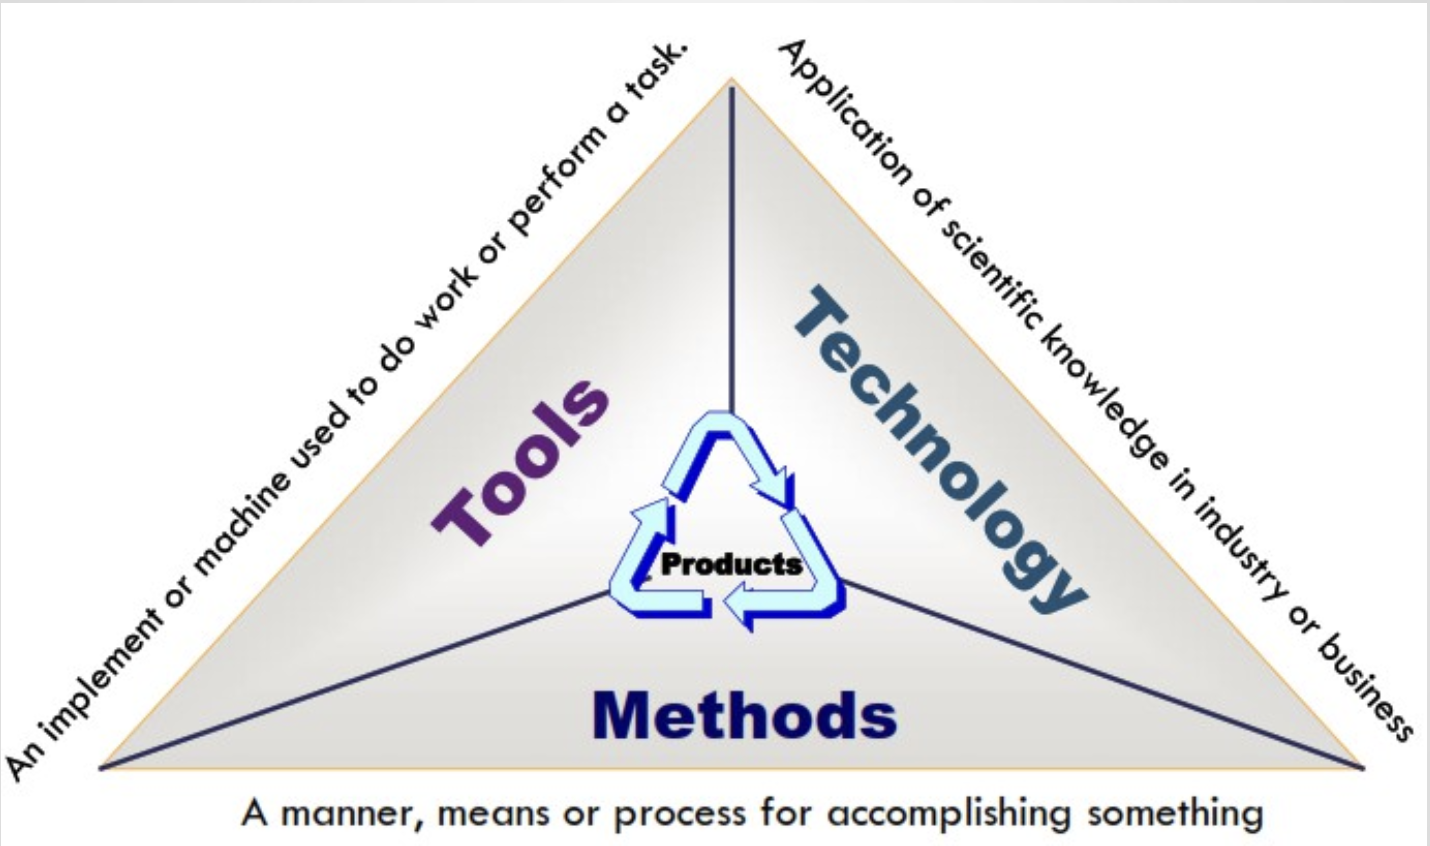
\includegraphics[width=7cm]{figures/swe-product.png}
\end{minipage}

\vspace{1ex}
\textbf{Essential attributes of good software:}
Maintainability, Efficiency, Acceptability, Dependability, Robustness, Integrity and Security
\subsection*{Difference between Program and Software Product}

\begin{tabularx}{\textwidth}{|X|X|}\hline
   \thc{Program} & \thc{Software Product} \\\hline
   Program is a set of instruction related each other. &
   Software Product is a collection of program designed for specific task. \\\hline
   Developed by individuals. & Developed by team. \\\hline
   Lack in proper documentation. &
   Proper documentation and well documented. \\\hline
   Development is Unplanned, not Systematic. &
   Developed in a planned, Systematic, organized approach. \\\hline
   Provides limited functionality and less features. &
   Provides more functionality and features \\\hline
\end{tabularx}

\subsection*{Cloud-Based Software Engineering}
Cloud computing is the delivery of on-demand computing services over
the internet on a pay-as-you-go basis.

\textbf{Most cloud computing services are:}
\begin{multicols}{2}
   \begin{enumerate}[parsep=0.5ex]
      \item Software as a service (SaaS)
      \item Platform as a service (PaaS)
      \item Infrastructure as a service (IaaS)
      \item Anything/Everything as a service (XaaS)
      \item Function as a Service (FaaS)
   \end{enumerate}
\end{multicols}
